\documentclass[review,3p]{elsarticle}
%\documentclass[5p]{elsarticle}

\usepackage{graphicx}               % Include figure files
\usepackage{array}
\usepackage{amsmath} 
\usepackage{amssymb} 
\usepackage{bm}                     % bold math
\usepackage{caption}
\usepackage{subcaption}
\usepackage{lineno}
\usepackage[mathcal]{euscript}
\usepackage{xcolor}                  % coloring text

\usepackage{lipsum}

\newcommand{\prtl}[2]{\frac{\partial #1}{\partial #2}}
%%%%%%%%%%%%%%%%%%%%%%%%%%%%%%%%%%%%%%%%%%%%%%%%%%%%%%%%%%%%%%%%%%%%%%%%%%%%%%%%%%%%

\begin{document}

%%%%%%%%%%%%%%%%%%%%%%%%%%%%%%%%%%%%%%%%%%%%%%%%%%%%%%%%%%%%%%%%%%%%%%%%%%%%%%%%%%%%

%\preprint{}

\title{Modeling Soot in Oxy-Coal Combustion Systems using Large Eddy Simulations}

\author[byu]{Kamron Brinkerhoff}
\author[lanl]{Alex Josephson}
\author[llnl]{Ben Isaac}
\author[uofu]{Jeremy Thornock}
\author[byu]{Andrew Fry}
\author[byu,*]{David Lignell\corref{cor1}}
\ead{davidlignell@byu.edu}

\address[byu]{350 CB, Brigham Young University, Provo, UT 84602, USA}
\address[lanl]{350 CB, Brigham Young University, Provo, UT 84602, USA}
\address[llnl]{350 CB, Brigham Young University, Provo, UT 84602, USA}
\address[uofu]{350 CB, Brigham Young University, Provo, UT 84602, USA}
\cortext[cor1]{Corresponding author}

\journal{Combustion and Flame}

\date{\today}

%%%%%%%%%%%%%%%%%%%%%%%%%%%%%%%%%%%%%%%%%%%%%%%%%%%%%%%%%%%%%%%%%%%%%%%%%%%%%%%%%%%%

\begin{abstract}

Soot in coal combustion simulations is often ignored due to its computational complexity, despite its significant effect on flame temperature and radiation.  In this research, a 40 kW oxy-coal combustion system is modeled using Large Eddy Simulations (LES) and a detailed monodisperse coal soot model. Cases where soot is modeled are compared with cases where soot is neglected to determine the accuracy benefits and computational costs of modeling soot.

\end{abstract}

\begin{keyword} 
Coal\sep Soot\sep LES\sep 
\end{keyword}

%-----------------------------------------------------------------------------------

\maketitle     

%-----------------------------------------------------------------------------------

\linenumbers

\section{Introduction}

%You can use the following cite commands:
%Single reference with number only: \cite{Zhao2013}
%Multiple references with number only: \cite{Affleck1967,Turanyi2014,uconnrcmpy}
%Single reference with two or fewer authors: \textcite{Affleck1967}
%Single reference with three or more authors: \textcite{Wang2011}
%Two references with authors: \textcite{Kee1996,Baumgardner2013}
%Three or more references with authors: \textcite{Kee1996,Baumgardner2013,Haworth2011}

	Coal currently provides 30\% of total energy worldwide \cite{DoE2019} 
but has an uncertain future due to concerns with with pollutants, especially carbon dioxide.  Methods to reduce carbon dioxide emmissions include cryogenic carbon capture \cite{Fazlollahi2015}, solvent absorption \cite{Yang2008}, and oxy-coal combustion.  While the first two examples separate CO2 from the flue gas, which is mainly nitrogen, oxy-coal combustion separates oxygen from nitrogen prior to combustion, and requires a much simpler separation of CO2 from water in the flue gas.   An additional benefit of oxy-combustion is that it reduces NO$_x$ formation since nitrogen is absent from the oxidizer stream.  

	Oxy-coal combustion has several obstacles that prevent its wide usage.  Separating oxygen from air is difficult, as it uses a great deal of energy and requires purchasing and installing additional equipment.  Using pure oxygen also alters combustion properties, such as soot concentration and flame temperature.  Since high temperatures cause combustor materials to fail, the flame must be cooled by recirculating exhaust gas to dilute the reactant stream \cite{Kather2009}.  This complicates designing oxy-coal facilities. 

	These difficulties have motivated researchers to develop computer simulations to help design oxy-coal combustion plants.  Although much can be learned from experiments, they are often unable to accurately measure all relevant combustion properties.  Simulations, if performed accurately, can provide considerably more detail than what could be measured in an experiment.  
 \section{Previous Work}
	 Most coal simulations use either Reynolds-Averaged Numerical Simulation (RANS), or Large Eddy Simulation (LES).  RANS averages all turbulent velocity fluctuations over time, sacrificing accuracy for low computational cost.  LES is more accurate but more computationally expensive, resolving large fluctuations or eddies while modeling smaller ones.  This compromise preserves the most important combustion details while still having lower computational costs compared to Direct Numerical Simulation, which resolves all turbulent fluctuations and is too computationally expensive for most coal combustion applications \citep{Luo2012}.  Several studies have documented the tradeoffs between LES and RANS  for coal combustion \citep{Yamamoto20111771} \citep{Gharebaghi2011} \citep{Edge2011} \citep{Stein2012} \citep{Warzecha2014732}.  Because of their differences, LES is often performed on smaller combustors compared to RANS.    
	
%TODO: Add jovanovic 2013,	
		
	
	The first coal LES simulations focused on generic solid-fuel combustion \citep{Kurose2003}, and subsequent simulations modeled oxy-coal jet flames \citep{Yamamoto20111771}, lab-scale burners\citep{Stein2012}, and industrial-sized burners \citep{Kurose2009} \citep{Gharebaghi2011}.  These simulations ignored soot formation due to the complexity of the tar precursors.  Because soot affects flame temperature through radiative heat transfer, other research has indicated that neglecting soot in simulations introduces significant error for coal-air flames \cite{Xu2017}\cite{Takahashi2019}.  Xu et al. \cite{Xu2017}, simulated coal soot formation in a jet flame using the mechanism proposed by Brown et al. \cite{Brown1998}.  They found that including soot formation decreased the flame temperature by about 238 K due to radiative heat loss.  Experimental measurements matched closest to the cases where soot was included, although the experimental temperatures were still slightly lower.  A similar study \cite{Takahashi2019} found that neglecting soot in a 4kw jet burner decreased flame temperature by 100 K.  The simulations proposed in this project will model soot in an pilot-scale oxy-coal combustor in preparation for future work, where we will determine soot's affect on temperature and flame properties by comparing current simulations with new simulations that neglect soot.  Since oxy-coal flames typically have more soot than air flames \cite{Stimpson2013}, neglecting soot would likely decrease temperature more than in an air-coal flame. 


\subsection{Soot Modeling}

	Our simulations will use a detailed monodisperse coal soot model recently developed by Josephson et. al.\cite{Josephson2019}.  Prior to this model's development, the most advanced coal soot model was the Brown model \cite{Brown1998}, a semiempirical model.  Josephson's improves on the Brown model in several ways. First, it models the soot processes that the Brown model neglects, i.e. soot surface growth, soot gasification, tar deposition, and tar cracking.  See table \ref{f:soot} for a schematic of soot processes.  Second, it utilizes collision rates derived from kinetic collision theory to calculate nucleation, coagulation, and tar deposition.  Third, it uses improved oxidation and gasification rates obtained using Bayesian statistics \cite{Josephson2017}.  
	%
%\begin{figure}[htpb]
  %  \centering
    %\includegraphics[width=4in]{soot_model_diagram2_bw.png}
    %\caption{Overview of soot processes}
    %\label{fig:soot}
%\end{figure}  
	
\begin{figure}
\begin{center}
\begin{tabular}{c}
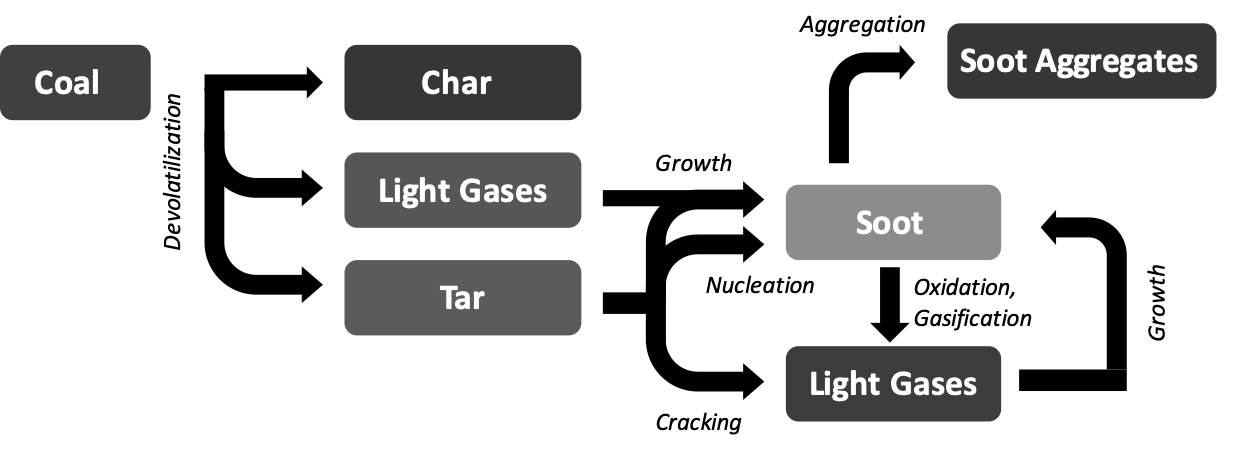
\includegraphics[width=4 in]{../figures/soot_model_Diagram2_bw.png}
\end{tabular}
\caption{Schematic of coal and soot processes}
\label{f:soot}
\end{center}
\end{figure}	

\subsection{Computational tools}
	This simulation will be run on Arches, a finite-volume LES code developed by the University of Utah, will be used for this project's simulations. It is parallelized on a C++ framework called Uintah.  It uses Message Passing Interface (MPI) to parallelize. Arches spatially and temporally solves mass, momentum, energy, and mixture fraction balances for low mach and variable density flows.  Favre filtering is used to remove small-scale turbulent fluctuations.  The dynamic Smagorinsky model is used to calculate the subgrid scale stress tensor.    It uses Direct Quadrature Method Of Moments (DQMOM) to represent coal particle size distributions  \cite{Pedel2012} \cite{Abboud2015} \cite{Marchisio2005}.  Arches uses the First Order With Yield (FOWY) model for coal devolatilization \cite{Schroeder2015}, the Smith model for char oxidation \cite{Smith1980}, and the discrete ordinates method to solve for radiation \cite{Modest2013541}.  


\subsection{Simulation Details}

The simulation will model the Oxy-Fuel Combustor (OFC) at BYU.  It will be validated using the experimental measurements of Stimpson et. al \cite{Stimpson2013}.  The OFC is a 1.7m long, 0.6m diameter reactor with a firing rate of 40 kW.  See Figure \ref{f:OFC} for a schematic.  Our simulation will include the burner zone of the reactor and the and the transition zone leading to the radiant section.  It uses Skyline coal with a stoichiometric ratio of 0.9.  The oxidizer stream is diluted with recycled $CO_2$ in order to reduce flame temperatures.  The simulation uses 21.5 million grid cells arranged as 425 X 225 X 225.  The simulation ran until it reached steady state after 7.5 seconds, after which it ran for another 5 seconds %(boundary/initial conditions?  )



\begin{figure}
\begin{center}
\begin{tabular}{c}
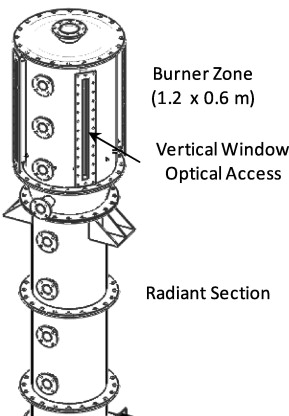
\includegraphics[width=2 in]{../figures/OFC_pic.jpg}
\end{tabular}
\caption{OFC schematic.}
\label{f:OFC}
\end{center}
\end{figure}




\begin{table}[h]
	\caption{Proximate Analysis.}
	\label{t:prox}
	\centering
	\begin{tabular}{l l l}
	\hline
	Component & wt\% \\ \hline
    Moisture & 3.18 \\ 
    Ash & 8.83 \\ 
    Volatile matter & 38.6  \\ 
    Fixed Carbon & 49.39  \\ 
\hline
\end{tabular}
\end{table}


\begin{table}[!h]
	\caption{Ultimate Analysis.}
	\label{t:ult}
	\centering
	\begin{tabular}{l l l}
	\hline
	Component & wt\% \\ \hline
	Carbon & 80.24 \\ 
    Hydrogen & 5.74 \\ 
    Nitrogen & 1.61 \\ \
    Sulfur & 0.60 \\ 
    Oxygen & 11.81 \\ 
\hline
\end{tabular}
\end{table}


\begin{table}[!h]
	\caption{Heating value (KJ/kg).}
	\label{t:heat}
	\centering
	\begin{tabular}{l l l}
	\hline
	
	As received & 29,321 \\ 
    Dry, ash free & 33,323 \\ 
\hline
\end{tabular}
\end{table}


\begin{table}[!h]
	\caption{Flow rate (kg/s).}
	\label{t:flowrates}
	\centering
	\begin{tabular}{l l l}
	\hline
	Stream & Flow Rate (kg/s)  \\ \hline
	Primary Coal & 1.242E-3  \\ 
    Primary $O_2$ & 3.432E-4\\ 
    Primary $CO_2$ & 2.210E-3  \\ 
    
    Secondary $O_2$ & 2.112E-3 \\ 
    Secondary $CO_2$ & 6.263E-3  \\ 
    Staging $O_2$ & 6.400E-4\\ 
    Staging $CO_2$ & 2.210E-3  \\
    Purge $CO_2$  & 1.065E-3  \\ 
	
\hline
\end{tabular}
\end{table}

The reactor uses 4 input streams whose names and flowrates are listed in table \ref{t:flowrates}.  The primary stream is a central tube entering the reactor and the secondary stream is an annulus surrounding the primary tub.  The staging stream is used to add extra oxygen near the exit to ensure that combustion products are fully oxidized.  Lastly, the purge stream is an inlet on the side of the reactor to prevent ash deposition on windows used for optical measurements.  

\begin{table}[!h]
	\caption{}
	\label{t:stream_temperatures}
	\centering
	\begin{tabular}{l l l}
	\hline
	Stream & Temperature(K) \\ \hline
    Primary & 366.5 \\ 
    Secondary & 529.4  \\ 
    Staging  & 294.2 \\ 
    Purge  & 294.2 \\ 
	
\hline
\end{tabular}
\end{table}



\section{Results and Discussion}
%
Figure \ref{f:results1} depicts flame properties in the central cross-section of the OFC.  
Note that the flame is quite lifted.  Soot appears to form prior to coal ignition as devolatilization begins, and most of the soot is oxidized before it can exit the flame.  Figure \ref{f:results2} depicts the same flame properties averaged over time.  Table \ref{t:temperatures} compare simulation flame temperatures with experimental measurements, showing close agreement with less than 3\% error.  Since the visualization software reports gas temperatures, they must be converted to the corresponding thermocouple temperatures when comparing with the experimental data.   Temperature corrections are calculated using Equation \ref{e:thermocouple}, and the results are included in table \ref{t:temperatures}.  Species concentrations, on the other hand, had larger errors, likely a result of incomplete char oxidation in the experiment that was not accurately represented in the simulation.  Table \ref{t:concentrations} depicts these values.  

\begin{figure}[!h]
\begin{center}
\begin{tabular}{c}
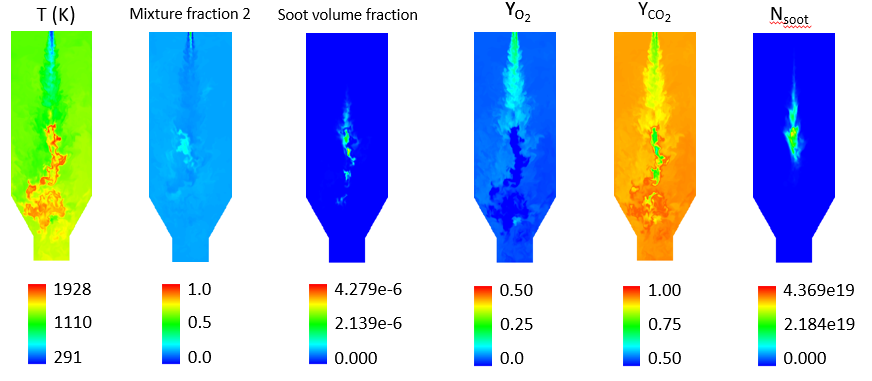
\includegraphics[width=6 in]{../figures/resultsB.png}
\end{tabular}
\caption{Instantaneous cross sections of the OFC after 12.5 seconds, where T(K) refers to temperature, Y refers to species mass fractions, and $N_{soot}$ refers to soot number density.  Mixture fraction 2 represents a stream consisting of mostly carbon dioxide and water }
\label{f:results1}
\end{center}
\end{figure}

\begin{figure}[!h]
\begin{center}
\begin{tabular}{c}
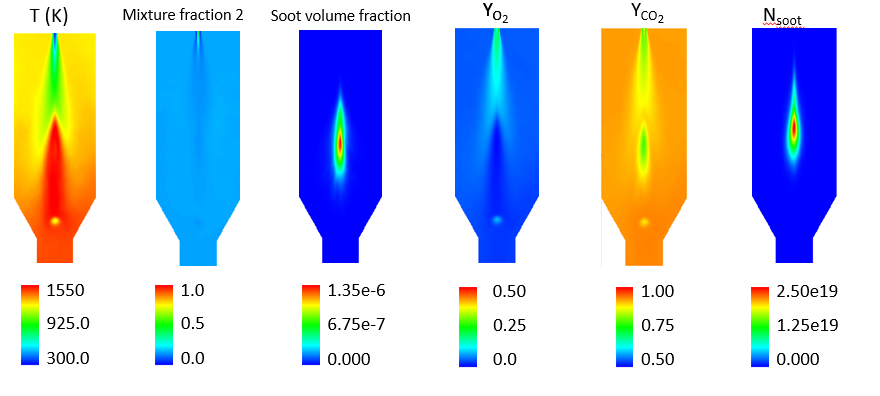
\includegraphics[width=6 in]{../figures/results_averaged.png}
\end{tabular}
\caption{ Time averaged cross sections of the OFC from 7.5 seconds to 12.5 seconds. }
\label{f:results2}
\end{center}
\end{figure}

\begin{equation} \label{e:thermocouple}
h_{C}(T_{g}-T_{t})=\epsilon\sigma(T_{t}^4-q_{in})\\.
\end{equation}

\begin{table}[!h]
	\caption{Where locations 1,2, and 3 refer to axial distances of 0.2m, 0.62m, and 1.02m respectively  }
	\label{t:temperatures}
	\centering
	\begin{tabular}{ | l | l | l | l |}
	\hline
       & location 1 & location 2 & location 3 \\ \hline
    Simulation (gas) & 1255.7 K & 1266.1 K & 1315.4 \\ 
    Simulation (thermocouple) & 1225.9 K & 1248.7 K & 1283.5 K \\ 
    Experiment (thermocouple) & 1249.5  K & 1287.5 K & 1281 K \\ 
    \hline
    \end{tabular}
\end{table}


\begin{table}[!h]
	\caption{Mass percentages at OFC exit }
	\label{t:concentrations}
	\centering
	\begin{tabular}{ | l | l | l | l |}
	\hline
	    & $CO_2$ & $O_2$   \\ \hline
    Simulation &  0.932 & 0.0288   \\ 
    Experiment  & 0.955 & 0.0336  \\  
\hline
\end{tabular}
\end{table}


 



Figure \ref{f:fvplot} depicts time-averaged line of sight soot measurements perpendicular to the reactor.  The simulation differs from the experiment by as much as an entire order of magnitude.  A possible explanation for this is that the flame in the simulation is more lifted than in the experiment, shifting the area of highest soot concentration farther down the reactor.  Although Stimpson et al \cite{Stimpson2013} indicated that the flame was lifted, they did not specify how much, and this uncertainty could affect soot concentration.  Alternatively, the error could be because of the inherent difficulty in accurately modeling and predicting soot concentrations for coal combustion, as errors in this field are often as large as an order of magnitude. 

\begin{figure}[!h] 
\begin{center}
\begin{tabular}{c}
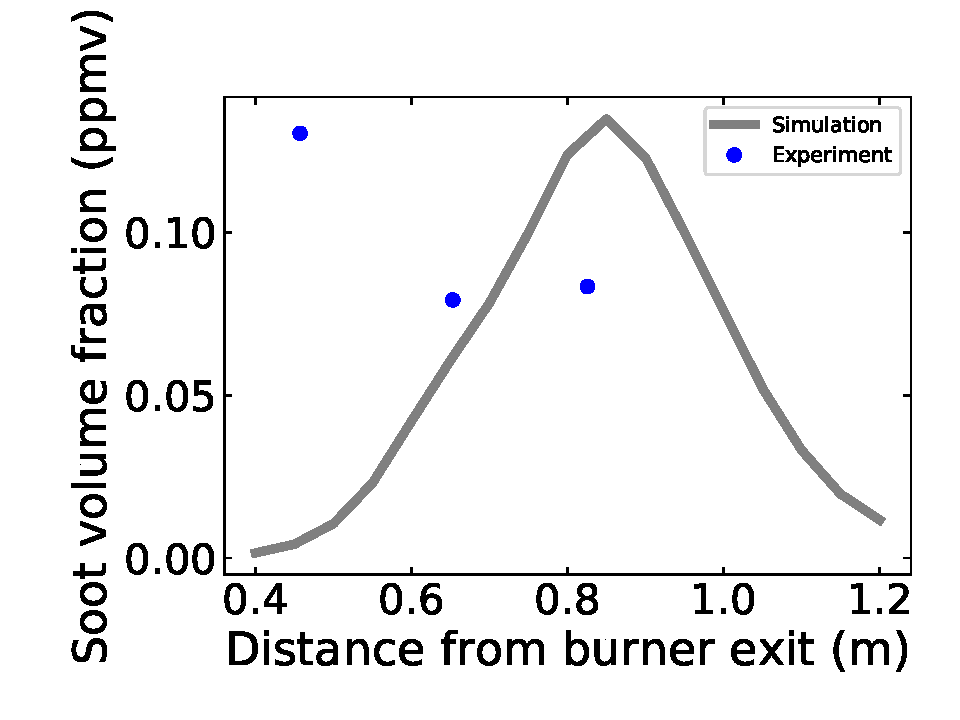
\includegraphics[width=4 in]{../figures/fv_plot/fv_plot.pdf}
\end{tabular}
\caption{   }
\label{f:fvplot}
\end{center}
\end{figure}

%--------------------------------------------------------------------------------

\section{Conclusions}
%
	Large Eddy Simulations of Oxy-coal combustion with soot formation included were performed with acceptable agreement with experimental data.  Areas of improvement include soot volume fraction, flame liftoff height, and oxygen concentrations at the burner exit.  Further research will compare current simulations with new simulations that neglect soot, in order to determine the effect of soot on flame temperature.

\section{Acknowledgements}
This work was supported by the Department of Energy, National Nuclear Security Administration under Award DE-NA0002375.

%\noindent\textbf{Page Limits:} The total length of the paper including references should be limited to 10 pages.

%%%%%%%%%%%%%%%%%%%%%%%%%%%%%%%%%%%%%%%%%%%%%%%%%%%%%%%%%%%%%%%%%%%%%%%%%%%%%%%%%%%%%

\bibliographystyle{elsarticle-num}
\bibliography{references}

%%%%%%%%%%%%%%%%%%%%%%%%%%%%%%%%%%%%%%%%%%%%%%%%%%%%%%%%%%%%%%%%%%%%%%%%%%%%%%%%%%%%

\end{document}
